% =====================================================================
% Mục 5. Phân tích phương sai hai chiều (Two-Way ANOVA)
%
% Gói cần có trong file chính: amsmath, amssymb, booktabs, tabularx, array,
%   caption, float, graphicx, listings, xcolor.
% Trước khi \input file này, file chính phải nạp các con số do code sinh ra:
%   % Generated by scripts/reports/report_anova_two_way.py; do not edit by hand.
\newcommand{\AnovaAlpha}{0{,}05}
\newcommand{\AnovaTotalCleaned}{2057}
\newcommand{\AnovaAtiDesktop}{77}
\newcommand{\AnovaAtiLaptop}{0}
\newcommand{\AnovaSampleN}{1980}
\newcommand{\AnovaDfErr}{1976}
\newcommand{\AnovaFCrit}{3{,}846}
\newcommand{\AnovaTCrit}{1{,}9612}
\newcommand{\AnovaCellAmdDesktopN}{677}
\newcommand{\AnovaCellAmdLaptopN}{117}
\newcommand{\AnovaCellNvidiaDesktopN}{1032}
\newcommand{\AnovaCellNvidiaLaptopN}{154}
\newcommand{\AnovaRawAmdDesktopMean}{137{,}28}
\newcommand{\AnovaRawAmdLaptopMean}{37{,}03}
\newcommand{\AnovaRawNvidiaDesktopMean}{138{,}06}
\newcommand{\AnovaRawNvidiaLaptopMean}{50{,}18}
\newcommand{\AnovaRawLaptopGapW}{13{,}15}
\newcommand{\AnovaRawAmdDesktopSd}{83{,}76}
\newcommand{\AnovaRawAmdLaptopSd}{28{,}26}
\newcommand{\AnovaRawLeveneW}{76{,}964}
\newcommand{\AnovaRawLeveneP}{$<$ 0{,}001}
\newcommand{\AnovaRawSdRatio}{2{,}96}
\newcommand{\AnovaRawShapiroW}{0{,}9707}
\newcommand{\AnovaRawShapiroP}{$<$ 0{,}001}
\newcommand{\AnovaRawMsErr}{5\,089{,}8}
\newcommand{\AnovaRawFMaker}{2{,}181}
\newcommand{\AnovaRawPMaker}{$=$ 0{,}1399}
\newcommand{\AnovaRawEtaMaker}{0{,}0011}
\newcommand{\AnovaRawFSeg}{397{,}709}
\newcommand{\AnovaRawPSeg}{$<$ 0{,}001}
\newcommand{\AnovaRawEtaSeg}{0{,}1675}
\newcommand{\AnovaRawEtaSegPct}{16{,}8}
\newcommand{\AnovaRawFInter}{1{,}718}
\newcommand{\AnovaRawPInter}{$=$ 0{,}1901}
\newcommand{\AnovaRawEtaInter}{0{,}0009}
\newcommand{\AnovaRawTukeyMinDeskLapW}{87{,}10}
\newcommand{\AnovaRawTukeyMaxDeskLapW}{101{,}04}
\newcommand{\AnovaRawWelchLaptopT}{-3{,}341}
\newcommand{\AnovaRawWelchLaptopP}{$<$ 0{,}001}
\newcommand{\AnovaRawWelchDesktopP}{$=$ 0{,}8401}
\newcommand{\AnovaLogLeveneW}{11{,}558}
\newcommand{\AnovaLogLeveneP}{$<$ 0{,}001}
\newcommand{\AnovaLogSdRatio}{1{,}23}
\newcommand{\AnovaLogShapiroW}{0{,}9622}
\newcommand{\AnovaLogShapiroP}{$<$ 0{,}001}
\newcommand{\AnovaLogAmdLapShapiroW}{0{,}9795}
\newcommand{\AnovaLogAmdLapShapiroP}{$=$ 0{,}0701}
\newcommand{\AnovaLogFMaker}{22{,}537}
\newcommand{\AnovaLogPMaker}{$<$ 0{,}001}
\newcommand{\AnovaLogEtaMaker}{0{,}0113}
\newcommand{\AnovaLogFSeg}{725{,}710}
\newcommand{\AnovaLogPSeg}{$<$ 0{,}001}
\newcommand{\AnovaLogEtaSeg}{0{,}2686}
\newcommand{\AnovaLogEtaSegPct}{26{,}9}
\newcommand{\AnovaLogFInter}{8{,}767}
\newcommand{\AnovaLogPInter}{$=$ 0{,}0031}
\newcommand{\AnovaLogEtaInter}{0{,}0044}
\newcommand{\AnovaGeomAmdDesktop}{108{,}4}
\newcommand{\AnovaGeomNvidiaDesktop}{117{,}5}
\newcommand{\AnovaGeomAmdLaptop}{28{,}2}
\newcommand{\AnovaGeomNvidiaLaptop}{39{,}9}
\newcommand{\AnovaLaptopGeomGapPct}{41{,}5}
\newcommand{\AnovaDesktopGeomGapPct}{8{,}4}
\newcommand{\AnovaLogTukeyDeskP}{$=$ 0{,}0796}
\newcommand{\AnovaLogTukeyLapP}{$<$ 0{,}001}
\newcommand{\AnovaLogMsErr}{0{,}4646}
\newcommand{\AnovaRawLsdSigCount}{4}
\newcommand{\AnovaLogLsdSigCount}{6}
\newcommand{\AnovaLogLsdDeskDiff}{0{,}0805}
\newcommand{\AnovaLogLsdDeskCrit}{0{,}0661}
\newcommand{\AnovaLogLsdLapDiff}{0{,}3474}
\newcommand{\AnovaLogLsdLapCrit}{0{,}1639}
\newcommand{\AnovaLogWelchDesktopP}{$=$ 0{,}0212}
\newcommand{\AnovaLogWelchLaptopP}{$<$ 0{,}001}

% (tạo bằng: python scripts/reports/report_anova_two_way.py).
% Không tham chiếu số mục hay số bảng của mục khác; gọi theo nội dung.
% =====================================================================

\subsection{Phân tích phương sai hai chiều}
\label{sec:anova_two_way}

\subsubsection{Đặt bài toán và giả thuyết kiểm định}

\textbf{Câu hỏi kiểm định:} \emph{Hãng sản xuất (\texttt{manufacturer}: Nvidia và AMD)
cùng phân khúc thiết bị (\texttt{segment}: Desktop và Laptop) có ảnh hưởng đến công suất
thiết kế tối đa của GPU rời hay không, và chênh lệch giữa hai hãng có phụ thuộc vào phân
khúc (hiệu ứng tương tác) hay không?} Với  mức ý nghĩa $\alpha = \AnovaAlpha$.

Theo mô hình ANOVA hai chiều có lặp :
\begin{equation}
  Y_{ijk} = \mu + \tau_i + \beta_j + (\tau\beta)_{ij} + \varepsilon_{ijk},
  \qquad \varepsilon_{ijk} \sim \mathcal{N}(0, \sigma^2)\ \text{độc lập},
  \label{eq:two_way_anova}
\end{equation}
{\sloppy với $i \in \{\text{AMD}, \text{Nvidia}\}$ ($a=2$), $j \in \{\text{Desktop},
\text{Laptop}\}$ ($b=2$), $N = \AnovaSampleN$, $df_E = N - ab = \AnovaDfErr$, cùng ràng buộc
$\sum_i \tau_i = \sum_j \beta_j = \sum_i (\tau\beta)_{ij} = \sum_j (\tau\beta)_{ij} = 0$.

Với cỡ mẫu không cân bằng, ta dùng \textbf{Type III SS} và bác bỏ $H_0$ khi $F >
f_{\alpha;\, df_1;\, df_E}$:\par}
\begin{itemize}\setlength{\itemsep}{1pt}\setlength{\parskip}{0pt}
  \item \textbf{Hãng ($SSG$):} $H_{0a}: \tau_1 = \tau_2 = 0$ đối với $H_{1a}: \exists i,\,
    \tau_i \neq 0$; bác bỏ khi $F_a = \mathrm{MSG}/\mathrm{MSE} >
    f_{\AnovaAlpha;\, 1;\, \AnovaDfErr}$.
  \item \textbf{Phân khúc ($SSB$):} $H_{0b}: \beta_1 = \beta_2 = 0$ đối với $H_{1b}:
    \exists j,\, \beta_j \neq 0$; bác bỏ khi $F_b = \mathrm{MSB}/\mathrm{MSE} >
    f_{\AnovaAlpha;\, 1;\, \AnovaDfErr}$.
  \item \textbf{Tương tác A$\times$B ($SSI$):} $H_{0ab}: (\tau\beta)_{ij} = 0\ \forall i,j$
    đối với $H_{1ab}: \exists (i,j),\, (\tau\beta)_{ij} \neq 0$; bác bỏ khi $F_{ab} =
    \mathrm{MSI}/\mathrm{MSE} > f_{\AnovaAlpha;\, 1;\, \AnovaDfErr}$.
\end{itemize}

\subsubsection{Xử lý dữ liệu}

{\sloppy Từ tập dữ liệu sau tiền xử lý gồm \AnovaTotalCleaned{} GPU rời đầy đủ các biến
bắt buộc, nhóm ATI ghi nhận \AnovaAtiDesktop{} quan sát ở phân khúc Desktop nhưng không
có quan sát nào ở phân khúc Laptop (\AnovaAtiLaptop{} mẫu), làm phát sinh ô khuyết và
không cho phép ước lượng đầy đủ hiệu ứng tương tác. Nhằm bảo đảm tính đầy đủ của mô hình
hai nhân tố $2 \times 2$ với các quan sát lặp tại mọi tổ hợp, phân tích chỉ giữ lại hai
hãng Nvidia và AMD ($N = \AnovaSampleN$, ô có cỡ mẫu nhỏ nhất đạt \AnovaCellAmdLaptopN{}
quan sát). Quy trình thiết lập giả thuyết, chuẩn bị mẫu, kiểm định ANOVA hai chiều và
tổng hợp kết luận được trình bày tại Đoạn code~\ref{lst:anova_call}.\par}

\begin{lstlisting}[language=Python, label={lst:anova_call},
  caption={Truyền dữ liệu đã làm sạch vào hàm chạy ANOVA hai chiều}]
cleaned = preprocess.load_analysis()
hyp = anova.build_gpu_power_hypotheses(alpha=0.05)
sample, col = anova.prepare_two_way_sample(
    cleaned, "max_power_w", "manufacturer", "segment",
    include_a=("Nvidia", "AMD"), log_transform=False,  # True cho thang log
)
res = anova.run_two_way_anova(
    sample, col, "manufacturer", "segment", ss_type="III"
)
conclusions = anova.conclude_two_way_anova(res, hyp)
\end{lstlisting}

\begin{table}[H]
  \centering
  \caption{Thống kê mô tả công suất GPU trên thang gốc (W) và thang logarit ($\ln$W),
    $n = \AnovaSampleN$}
  \label{tab:anova_cells}
  \scriptsize
  \setlength{\tabcolsep}{3pt}
  \begin{tabular}{@{}lrcrrrr@{}}
    \toprule
    \textbf{Tổ hợp} & \textbf{$n$} & \textbf{Gốc: TB $\pm$ SD}
      & \textbf{Trung vị} & \textbf{Log: TB $\pm$ SD}
      & \textbf{TB nhân (W)} & \textbf{Shapiro $W$ ($p$)$^*$} \\
    \midrule
    \csname @@input\endcsname generated/anova_cells_combined.tex
    \bottomrule
    \multicolumn{7}{@{}p{\linewidth}@{}}{\scriptsize $^*$ Kiểm định Shapiro--Wilk theo
      từng ô trên thang log; trên thang gốc cả bốn ô đều cho $p < 0{,}001$.}
  \end{tabular}
\end{table}

\textbf{Nhận xét Bảng~\ref{tab:anova_cells}.} Công suất trung bình của GPU Desktop ở AMD
(\AnovaRawAmdDesktopMean{}~W) và Nvidia (\AnovaRawNvidiaDesktopMean{}~W) vượt trội rõ rệt
so với phân khúc Laptop (\AnovaRawAmdLaptopMean{}~W và \AnovaRawNvidiaLaptopMean{}~W).
Trong phân khúc Desktop, mức công suất trung bình giữa hai hãng gần như tương đương; ngược
lại, ở phân khúc Laptop, Nvidia cao hơn AMD \AnovaRawLaptopGapW{}~W (trung bình nhân
\AnovaGeomNvidiaLaptop{}~W so với \AnovaGeomAmdLaptop{}~W, cao hơn
\AnovaLaptopGeomGapPct{}\%), gợi ý khả năng tồn tại hiệu ứng tương tác giữa hãng và phân
khúc.

\begin{figure}[H]
  \centering
  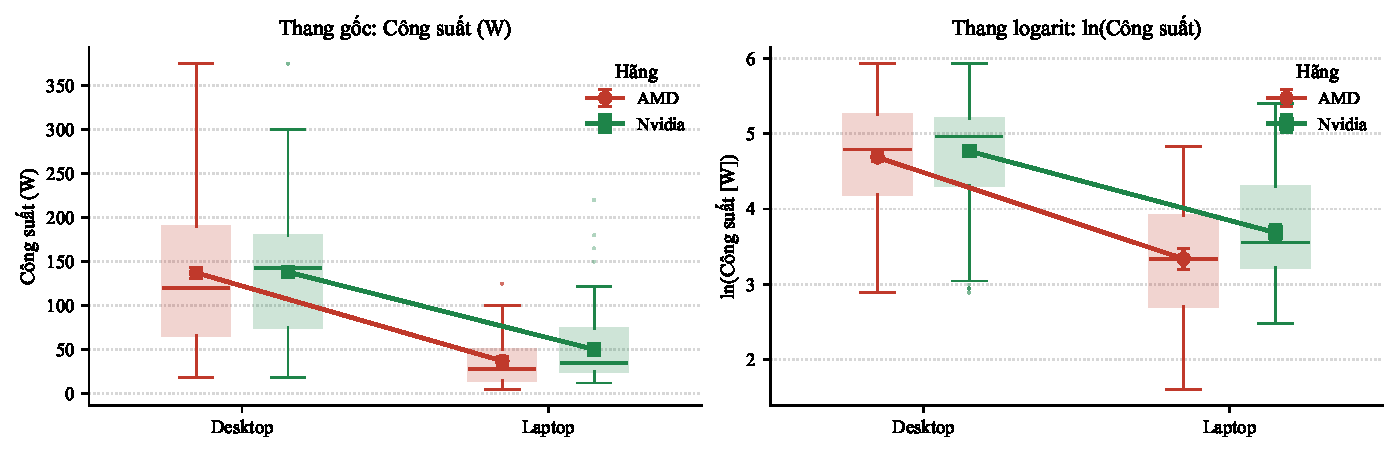
\includegraphics[width=\linewidth]{figures/anova_interaction.pdf}
  \caption{Biểu đồ hộp và đường tương tác trung bình (khoảng tin cậy 95\%) trên thang gốc
    (trái) và thang logarit (phải)}
  \label{fig:anova_interaction}
\end{figure}

\textbf{Nhận xét Hình~\ref{fig:anova_interaction}.} Thang gốc có độ rộng hộp nhóm Desktop
lớn hơn hẳn Laptop và lệch phải mạnh ($\text{SD}_{\max}/\text{SD}_{\min} =
\AnovaRawSdRatio$). Biến đổi logarit làm độ trải bốn nhóm đồng đều hơn rõ rệt và cho thấy
hai đường trung bình không song song (khoảng cách ở Laptop rộng hơn Desktop).

\subsubsection{Kiểm tra giả định và kết quả ANOVA hai chiều}

{\sloppy \textbf{Kiểm tra ba giả định ANOVA.}

\textbf{(1) Tính chuẩn:} trên thang gốc, Shapiro--Wilk bác bỏ ở bốn ô và phần dư
($W = \AnovaRawShapiroW$, $p$~\AnovaRawShapiroP); trên thang log, ô AMD -- Laptop thỏa
chuẩn ($p$~\AnovaLogAmdLapShapiroP), còn phần dư lệch nhẹ do $n$ lớn
($W = \AnovaLogShapiroW$, $p$~\AnovaLogShapiroP) nhưng $n_{ij} \ge
\AnovaCellAmdLaptopN$ bảo đảm kiểm định $F$ bền vững.

\textbf{(2) Đồng nhất phương sai:} Levene thang gốc bác bỏ mạnh
($W = \AnovaRawLeveneW$, $p$~\AnovaRawLeveneP, tỉ số SD $= \AnovaRawSdRatio$); thang log
đưa tỉ số SD còn \textbf{\AnovaLogSdRatio{}} ($< 2{,}0$) và giảm $W$ xuống
$\AnovaLogLeveneW$ ($p$~\AnovaLogLeveneP).

\textbf{(3) Tính độc lập:} các bản ghi ứng với mẫu GPU độc lập, song một số card dùng
chung kiến trúc nên kết quả được kiểm chứng thêm bằng Welch $t$-test.\par}

\begin{table}[H]
  \centering
  \caption{Kết quả ANOVA hai chiều (Type III SS) trên thang gốc và thang logarit
    ($\alpha = \AnovaAlpha$, $f_{\AnovaAlpha;\, 1;\, \AnovaDfErr} = \AnovaFCrit$)}
  \label{tab:anova_table}
  \footnotesize
  \setlength{\tabcolsep}{4pt}
  \begin{tabular}{@{}lrrrrrr@{}}
    \toprule
    \textbf{Nguồn biến thiên} & \textbf{$SS$} & \textbf{$df$} & \textbf{$MS$}
      & \textbf{$F$} & \textbf{$p$-value} & \textbf{$\eta_p^2$} \\
    \midrule
    \csname @@input\endcsname generated/anova_table_combined.tex
    \bottomrule
    \multicolumn{7}{@{}p{\linewidth}@{}}{\scriptsize $^*$ Với Type III SS cho cỡ mẫu không
      cân bằng, tổng $SSG + SSB + SSI + SSE$ nói chung khác $SST$.}
  \end{tabular}
\end{table}

\textbf{Nhận xét Bảng~\ref{tab:anova_table}.}\\
\textbf{-- Trên thang gốc (Panel A):} chỉ có yếu tố \textbf{phân khúc} ảnh hưởng có ý
nghĩa thống kê ($F_b = \AnovaRawFSeg > \AnovaFCrit$, $p$~\AnovaRawPSeg, giải thích
$\eta_p^2 = \AnovaRawEtaSeg$, tương đương \AnovaRawEtaSegPct{}\% phương sai cục bộ),
do đó bác bỏ $H_{0b}$. Ngược lại, yếu tố \textbf{hãng} ($F_a = \AnovaRawFMaker \le
\AnovaFCrit$, $p$~\AnovaRawPMaker) và \textbf{tương tác} ($F_{ab} = \AnovaRawFInter \le
\AnovaFCrit$, $p$~\AnovaRawPInter) đều chưa đủ cơ sở bác bỏ $H_{0a}$ và $H_{0ab}$; nguyên
nhân là độ phân tán công suất trong nhóm Desktop rất lớn làm phương sai sai số
($\mathrm{MSE} = \AnovaRawMsErr$) tăng cao, che lấp khác biệt giữa hai hãng.\\
\textbf{-- Trên thang logarit (Panel B):} sau khi ổn định phương sai
($\mathrm{MSE} = \AnovaLogMsErr$), cả ba thống kê $F$ đều lớn hơn ngưỡng tới hạn
$\AnovaFCrit$ nên bác bỏ đồng thời $H_{0a}$, $H_{0b}$ và $H_{0ab}$. Cụ thể,
\textbf{phân khúc} vẫn là nhân tố chi phối mạnh nhất ($F_b = \AnovaLogFSeg$,
$p$~\AnovaLogPSeg, giải thích \AnovaLogEtaSegPct{}\% phương sai cục bộ), bên cạnh tác
động chính của \textbf{hãng sản xuất} ($F_a = \AnovaLogFMaker$, $p$~\AnovaLogPMaker) và
\textbf{hiệu ứng tương tác có ý nghĩa thống kê} ($F_{ab} = \AnovaLogFInter$,
$p$~\AnovaLogPInter).

\subsubsection{Phân tích Hậu kiểm}

{\sloppy \textbf{(1) Hậu kiểm Fisher's LSD.} Trên thang gốc, Fisher's LSD chỉ phát hiện
\AnovaRawLsdSigCount/6 cặp khác biệt (đều là các cặp giữa Desktop và Laptop; hai hãng
không khác biệt trong từng phân khúc). Trên thang logarit ($\mathrm{MSE} = \AnovaLogMsErr$),
phương pháp này phát hiện cả \AnovaLogLsdSigCount/6 cặp đều khác biệt, gồm cả cặp Laptop
($|\Delta| = \AnovaLogLsdLapDiff > \AnovaLogLsdLapCrit$) và cặp Desktop
($|\Delta| = \AnovaLogLsdDeskDiff > \AnovaLogLsdDeskCrit$). \emph{Lý do cần kiểm chứng
thêm:} Fisher's LSD chỉ giữ mức sai số loại I bằng $\alpha = \AnovaAlpha$ cho từng cặp
riêng lẻ chứ không hiệu chỉnh cho cả họ 6 phép so sánh cùng lúc, nên nguy cơ báo khác biệt
giả (dương tính giả) tăng cao ở những cặp có độ lệch nhỏ như cặp Desktop.\par}

{\sloppy \textbf{(2) Hậu kiểm Tukey HSD.} Để khắc phục hiện tượng phồng sai số loại I khi
so sánh bội của Fisher's LSD, nhóm áp dụng thêm Tukey HSD nhằm kiểm soát sai số loại I
đồng thời trên toàn bộ 6 cặp ở đúng mức $\alpha = \AnovaAlpha$
(Hình~\ref{fig:anova_tukey_ci}).\par}

\begin{figure}[H]
  \centering
  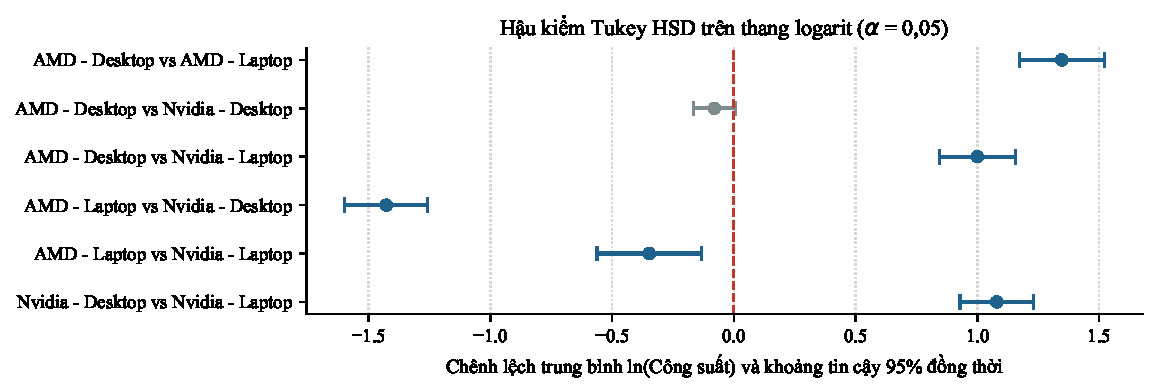
\includegraphics[width=\linewidth]{figures/anova_tukey_ci.pdf}
  \caption{Khoảng tin cậy 95\% đồng thời của hậu kiểm Tukey HSD trên thang logarit}
  \label{fig:anova_tukey_ci}
\end{figure}

\textbf{Nhận xét Hình~\ref{fig:anova_tukey_ci}.} Sau khi hiệu chỉnh bội bằng Tukey HSD
trên thang logarit, có 5/6 cặp sở hữu khoảng tin cậy 95\% đồng thời không chứa 0
($p < 0{,}001$). Riêng cặp AMD -- Desktop so với Nvidia -- Desktop bị cắt qua 0
($p$~\AnovaLogTukeyDeskP), cho thấy chênh lệch rất nhỏ ở phân khúc Desktop mà Fisher's LSD
ghi nhận không còn đủ ý nghĩa thống kê khi kiểm soát sai số toàn họ. Ngược lại, trên
Laptop, Nvidia vẫn cao hơn AMD rõ rệt ($p$~\AnovaLogTukeyLapP), khẳng định trực tiếp nguồn
gốc của hiệu ứng tương tác giữa hãng và phân khúc.

{\sloppy \textbf{(3) Kiểm chứng hiệu ứng đơn bằng Welch $t$-test.} Do mô hình có hiệu ứng
tương tác và kiểm định Levene vẫn ghi nhận khác biệt phương sai giữa các ô, các phương
pháp dùng phương sai gộp ($\mathrm{MSE}$) như ANOVA, Fisher's LSD hay Tukey HSD có thể
bị ảnh hưởng trên thang gốc. Vì vậy, nhóm thực hiện thêm kiểm định hiệu ứng đơn (cố định
từng mức của một nhân tố để so sánh nhân tố còn lại) bằng \textbf{Welch $t$-test} --
phương pháp không đòi hỏi hai nhóm có phương sai bằng nhau
(Bảng~\ref{tab:anova_simple_effects}).\par}

\begin{table}[H]
  \centering
  \caption{Kiểm định hiệu ứng đơn bằng Welch $t$-test (không cần phương sai bằng nhau)}
  \label{tab:anova_simple_effects}
  \footnotesize
  \setlength{\tabcolsep}{3.5pt}
  \begin{tabular}{@{}llrrrrrr@{}}
    \toprule
    & & \multicolumn{3}{c}{\textbf{Thang gốc (W)}}
      & \multicolumn{3}{c}{\textbf{Thang logarit ($\ln$W)}} \\
    \cmidrule(lr){3-5} \cmidrule(lr){6-8}
    \textbf{Điều kiện} & \textbf{Cặp so sánh} & \textbf{Chênh lệch} & \textbf{$t$}
      & \textbf{$p$-value} & \textbf{Chênh lệch} & \textbf{$t$} & \textbf{$p$-value} \\
    \midrule
    \csname @@input\endcsname generated/anova_simple_effects.tex
    \bottomrule
  \end{tabular}
\end{table}

\textbf{Nhận xét Bảng~\ref{tab:anova_simple_effects}.} Kết quả Welch $t$-test nhất quán
trên cả hai thang đo và củng cố trực tiếp kết luận tương tác:\\
\textbf{-- So sánh phân khúc trong từng hãng:} công suất GPU Desktop luôn cao hơn Laptop
rất mạnh ở cả AMD lẫn Nvidia ($p < 0{,}001$).\\
\textbf{-- So sánh hai hãng trong nhóm Laptop:} khi tách riêng phương sai của nhóm Laptop
(không bị độ phân tán lớn của Desktop kéo $\mathrm{MSE}$ lên cao), Nvidia cao hơn AMD rõ
rệt ngay cả trên thang gốc ($t = \AnovaRawWelchLaptopT$, $p$~\AnovaRawWelchLaptopP) lẫn
thang logarit ($p$~\AnovaLogWelchLaptopP), chứng tỏ chênh lệch này là bản chất thật của
dữ liệu chứ không do phép biến đổi logarit tạo ra.\\
\textbf{-- So sánh hai hãng trong nhóm Desktop:} hai hãng gần như tương đương trên thang
gốc ($p$~\AnovaRawWelchDesktopP) và chỉ lệch rất nhẹ trên thang logarit
($p$~\AnovaLogWelchDesktopP, không còn ý nghĩa thống kê sau khi hiệu chỉnh so sánh bội
bằng Tukey HSD).

\subsubsection{Kết luận}

Từ kết quả phân tích phương sai hai chiều ở mức ý nghĩa $\alpha = \AnovaAlpha$, có thể
trả lời trực tiếp câu hỏi kiểm định như sau: Trên thang logarit (thang đo
chính đã ổn định phương sai), dữ liệu có đủ bằng chứng thống kê để bác bỏ đồng thời cả ba giả
thuyết không $H_{0a}$, $H_{0b}$ và $H_{0ab}$. Điều này khẳng định cả \textbf{hãng sản
xuất} ($p$~\AnovaLogPMaker), \textbf{phân khúc thiết bị} ($p$~\AnovaLogPSeg) và
\textbf{hiệu ứng tương tác giữa hai yếu tố} ($p$~\AnovaLogPInter) đều ảnh hưởng có ý
nghĩa đến công suất thiết kế tối đa của GPU rời (trong khi trên thang gốc chỉ bác bỏ được
$H_{0b}$ do phương sai rất lớn ở phân khúc Desktop che lấp khác biệt giữa hai hãng). Cụ thể, kết quả phân tích cho thấy ba điểm chính: 

\textbf{(1) Nhân tố chi phối chính:} phân khúc thiết bị là nguồn biến thiên lớn nhất, giải
thích \AnovaRawEtaSegPct{}\%--\AnovaLogEtaSegPct{}\% phương sai cục bộ, với công suất GPU
Desktop luôn cao hơn vượt trội so với Laptop ở cả hai hãng.

\textbf{(2) Bản chất hiệu ứng tương tác:} chênh lệch giữa hai hãng phụ thuộc rõ rệt vào
phân khúc -- ở phân khúc Desktop, Nvidia và AMD gần như tương đương (trung bình nhân
\AnovaGeomNvidiaDesktop{}~W so với \AnovaGeomAmdDesktop{}~W, không có ý nghĩa theo Tukey
HSD); ngược lại, ở phân khúc Laptop, Nvidia cao hơn AMD \AnovaLaptopGeomGapPct{}\% (trung
bình nhân \AnovaGeomNvidiaLaptop{}~W so với \AnovaGeomAmdLaptop{}~W).

\textbf{(3) Hạn chế và hướng phân tích tiếp theo:} một số mẫu GPU dùng chung kiến trúc
chip (\texttt{architecture}) nên giả định độc lập giữa các quan sát chỉ mang tính gần
đúng, song toàn bộ kết luận chính đều bền vững khi kiểm chứng bằng Welch $t$-test. Đồng
thời, do phần lớn biến thiên công suất vẫn nằm trong nội bộ phân khúc Desktop, mô hình
hồi quy ở mục tiếp theo sẽ bổ sung các biến thông số phần cứng định lượng để giải thích
đầy đủ hơn công suất GPU.
